\documentclass{beamer}

% Setup appearance:

\usetheme{Darmstadt}
\usefonttheme[onlylarge]{structurebold}
\setbeamerfont*{frametitle}{size=\normalsize,series=\bfseries}
\setbeamertemplate{navigation symbols}{}


% Standard packages

\usepackage[brazil]{babel}
\usepackage[latin1]{inputenc}
\usepackage{times}
\usepackage[T1]{fontenc}
\usepackage[table]{xcolor}
 
% Setup TikZ

\usepackage{tikz}
\usetikzlibrary{arrows}
\tikzstyle{block}=[draw opacity=0.7,line width=1.4cm]

%diret\'orio das figuras
\graphicspath{../article}

\title[Filtro El\'iptico]{%
Filtro El\'iptico%
}

\author[Souza,Santos,Ara\'ujo]{
     Danilo~Souza\and
     Hugo~Santos\and
     Welton~Ara\'ujo
     }
 

\institute[Bel\'em]{
  \inst{1}%
  Universidade Federal do Par\'a
  }
\date[Bel\'em 2012]{
  03 de Julho de 2012
  }



\begin{document}

\begin{frame}
  \titlepage
\end{frame}

\begin{frame}{Agenda}
  \tableofcontents
\end{frame}

\section{Introdu\c{c}\~ao}
\begin{frame}{Filtros Digitais}
	\begin{itemize}
	 \item	Filtros FIR
	 \item	Filtros IIR
		\begin{itemize}
		  \item Mapemamento de filtros anal\'ogicos
		  \item Menor ordem
		  \item Mais dif\'iceis de projetar
		  \item Problemas com Estabilidade
		\end{itemize}
	\end{itemize}
\end{frame}



\section{Filtro El\'iptico}
<<<<<<< HEAD

	
=======
>>>>>>> 9bd42971d433320de75bcb48247ad5093a031aa9
	\begin{frame}{Filtro El\'iptico}
		\begin{itemize}
			\item Maior declive na banda de transi\c{c}\~ao
			\item Menor ordem que outros filtros IIR
			\item N\~ao possui fase linear
			\item Projetado somente em termos de magnitude
		\end{itemize}
	\end{frame}




\subsection{Projeto de Filtros El\'ipticos}
   
	\begin{frame}{Abordagens}
		\begin{itemize}
			\item Duas abordagens
		\end{itemize}
		\begin{itemize}
			\item  Abordagem I
				\begin{itemize}
					\item Projetar filtro Passa-Baixa anal\'ogico
					\item Realizar transforma\c{c}\~ao em frequ\^encia (s \(\rightarrow\) s)
					\item Aplicar transforma\c{c}\~ao do filtro (s \(\rightarrow\) z)
				\end{itemize}
	\end{itemize}
		\begin{itemize}
			\item Abordagem II
				\begin{itemize}
					\item Projetar filtro Passa-Baixa anal\'ogico
					\item Aplicar transforma\c{c}\~ao do filtro (s \(\rightarrow\) z)
					\item Realizar transforma\c{c}\~ao em frequ\^encia (z \(\rightarrow\) z)
				\end{itemize}
		\end{itemize}
	\end{frame}

\subsubsection{Projeto do filtro}
	\begin{frame}{Projeto dos filtros}
		\begin{itemize}
		 \item Encontrar a frequ\^encia digital \omega
		\end{itemize}
		\begin{itemize}
		 \item Encontrar a frequ\^encia distorcida \Omega
		\end{itemize}
		\begin{itemize}
		 \item \'E preciso encontrar algumas constantes para calcular a ordem do filtro
		\end{itemize}
	\end{frame}
	
<<<<<<< HEAD
\subsubsection{Tranforma\c{c}\~ao em Frequ\^encia}
=======
\subsubsection{Tranforma\c{c}\~ao em Freque\^encia}
>>>>>>> 9bd42971d433320de75bcb48247ad5093a031aa9
	\begin{frame}
		\begin{itemize}
		 \item Filtro passa-baixa
			  \begin{equation}
			  s' \leftrightarrow \frac{1}{a} \frac{s}{\Omega_{p}}
			  \end{equation}
		 \item Filtro rejeita-faixa
			  \begin{equation}
			  s' \leftrightarrow \frac{1}{a} \frac{B_{s}}{s^{2} + \Omega_{0}^{2}}
			  \end{equation}
		\end{itemize}

	\end{frame}
	
\subsubsection{Tranforma\c{c}\~ao Bilinear}

	\begin{frame}
		\begin{itemize}
			\item Mapear o plano \textit{s} para o plano \textit{z}
				\begin{itemize}
<<<<<<< HEAD
				\item  		\[s = \frac{1+z(T/2)}{1-z(T/2)}\]
=======
				\item  		\[z = \frac{1+s(T/2)}{1-s(T/2)}\]
>>>>>>> 9bd42971d433320de75bcb48247ad5093a031aa9
				\end{itemize}
			\item Mapear o eixo \textit{jw} para a circunfer\^encia de raio unit\'ario
			\item Mapear o lado esquerdo do plano \textit{s} para o interior da circunfer\^encia de raio unit\'ario
			\item Mapear o lado direto do plano \textit{s} para o exterior da circunfer\^encia de raio unit\'ario
			\item Compress\~ao das frequ\^encias (\textit{warping})
			\item \(-\infty < \Omega < \infty\) para \(-\pi < \omega < \pi\)
		\end{itemize}

	\end{frame}
	

\section{A Implementa\c{c}\~ao}
	\begin{frame}{Requisitos dos filtros}
		\begin{table}[ht]
		%\centering
			\begin{tabular}{|l|l|}
				\hline
				\(A_p\) 	& 1 dB		\\ \hline
				\(A_r\) 	& 40 dB		\\ \hline
				\(\Omega_p\) 	& 1000 Hz	\\ \hline
				\(\Omega_r\) 	& 1290 Hz	\\ \hline
				\(\Omega_s\) 	& 3000 Hz	\\ \hline
			\end{tabular}
			\label{tab:tabfiltro1}\quad
		%\end{table}%
		
		%\begin{table}[ht]
		%\centering
			\begin{tabular}{|l|l|}
				\hline
				\(A_p\) 	& 0,5 dB	\\ \hline
				\(A_r\) 	& 60 dB		\\ \hline
				\(\Omega_p1\) 	& 40 rad/s	\\ \hline
				\(\Omega_r1\) 	& 50 rad/s	\\ \hline
				\(\Omega_r2\) 	& 70 rad/s	\\ \hline
				\(\Omega_p2\) 	& 80 rad/s	\\ \hline
				\(\Omega_s\) 	& 240 rad/s	\\ \hline
			\end{tabular}
			\label{tab:tabfiltro2}
		\end{table}

	\end{frame}
  
\subsection{Resultados}

\subsubsection{Filtro I}
<<<<<<< HEAD
	\begin{frame}{Resposta em magnitude - Filtro I}
		\begin{figure}[ht]
			\centering
			\includegraphics[width=9cm]{../pictures/Filtro1/RespMagnitudeFiltro1.png}
			\label{fig:magnitude1}
		\end{figure}
	\end{frame}
	\begin{frame}{Resposta em Fase - Filtro I}
		\begin{figure}[ht]
			\centering
			\includegraphics[width=9cm]{../pictures/Filtro1/RespFaseFiltro1.png}
			\label{fig:magnitude1}
		\end{figure}
	\end{frame}
	\begin{frame}{Resposta ao Impulso - Filtro I}
		\begin{figure}[ht]
			\centering
			\includegraphics[width=9cm]{../pictures/Filtro1/RespImpulsoFiltro1.png}
			\label{fig:magnitude1}
		\end{figure}
	\end{frame}
	\begin{frame}{Diagrama de polos e zeros - Filtro I}
		\begin{figure}[ht]
			\centering
			\includegraphics[width=9cm]{../pictures/Filtro1/DiagramaFiltro1.png}
=======
	\begin{frame}{Resposta em magnitude}
		\begin{figure}[ht]
			\centering
			\includegraphics[width=9cm]{..pictures/Filtro1/RespMagnitudeFiltro1.png}
			\label{fig:magnitude1}
		\end{figure}
	\end{frame}
	\begin{frame}{Resposta em Fase}
		\begin{figure}[ht]
			\centering
			\includegraphics[width=9cm]{..pictures/Filtro1/RespFaseFiltro1.png}
			\label{fig:magnitude1}
		\end{figure}
	\end{frame}
	\begin{frame}{Resposta ao Impulso}
		\begin{figure}[ht]
			\centering
			\includegraphics[width=9cm]{..pictures/Filtro1/RespImpulsoFiltro1.png}
			\label{fig:magnitude1}
		\end{figure}
	\end{frame}
	\begin{frame}{Diagrama de polos e zeros}
		\begin{figure}[ht]
			\centering
			\includegraphics[width=9cm]{..pictures/Filtro1/DiagramaFiltro1.png}
>>>>>>> 9bd42971d433320de75bcb48247ad5093a031aa9
			\label{fig:magnitude1}
		\end{figure}
	\end{frame}

\subsubsection{Filtro II}
<<<<<<< HEAD
	\begin{frame}{Resposta em magnitude - Filtro II}
		\begin{figure}[ht]
			\centering
			\includegraphics[width=9cm]{../pictures/Filtro2/RespMagnitudeFiltro2.png}
			\label{fig:magnitude1}
		\end{figure}
	\end{frame}
	\begin{frame}{Resposta em Fase - Filtro II}
		\begin{figure}[ht]
			\centering
			\includegraphics[width=9cm]{../pictures/Filtro2/RespFaseFiltro2.png}
			\label{fig:magnitude1}
		\end{figure}
	\end{frame}
	\begin{frame}{Resposta ao Impulso - Filtro II}
		\begin{figure}[ht]
			\centering
			\includegraphics[width=9cm]{../pictures/Filtro2/RespImpulsoFiltro2.png}
			\label{fig:magnitude1}
		\end{figure}
	\end{frame}
	\begin{frame}{Diagrama de polos e zeros - Filtro II}
		\begin{figure}[ht]
			\centering
			\includegraphics[width=9cm]{../pictures/Filtro2/DiagramaFiltro2.png}
=======
	\begin{frame}{Resposta em magnitude}
		\begin{figure}[ht]
			\centering
			\includegraphics[width=9cm]{..pictures/Filtro2/RespMagnitudeFiltro2.png}
			\label{fig:magnitude1}
		\end{figure}
	\end{frame}
	\begin{frame}{Resposta em Fase}
		\begin{figure}[ht]
			\centering
			\includegraphics[width=9cm]{..pictures/Filtro2/RespFaseFiltro2.png}
			\label{fig:magnitude1}
		\end{figure}
	\end{frame}
	\begin{frame}{Resposta ao Impulso}
		\begin{figure}[ht]
			\centering
			\includegraphics[width=9cm]{..pictures/Filtro2/RespImpulsoFiltro2.png}
			\label{fig:magnitude1}
		\end{figure}
	\end{frame}
	\begin{frame}{Diagrama de polos e zeros}
		\begin{figure}[ht]
			\centering
			\includegraphics[width=9cm]{..pictures/Filtro2/DiagramaFiltro2.png}
>>>>>>> 9bd42971d433320de75bcb48247ad5093a031aa9
			\label{fig:magnitude1}
		\end{figure}
	\end{frame}
	
\end{document}
